\vspace*{-3cm}\textbf{}\\
\hspace*{-2.5cm}
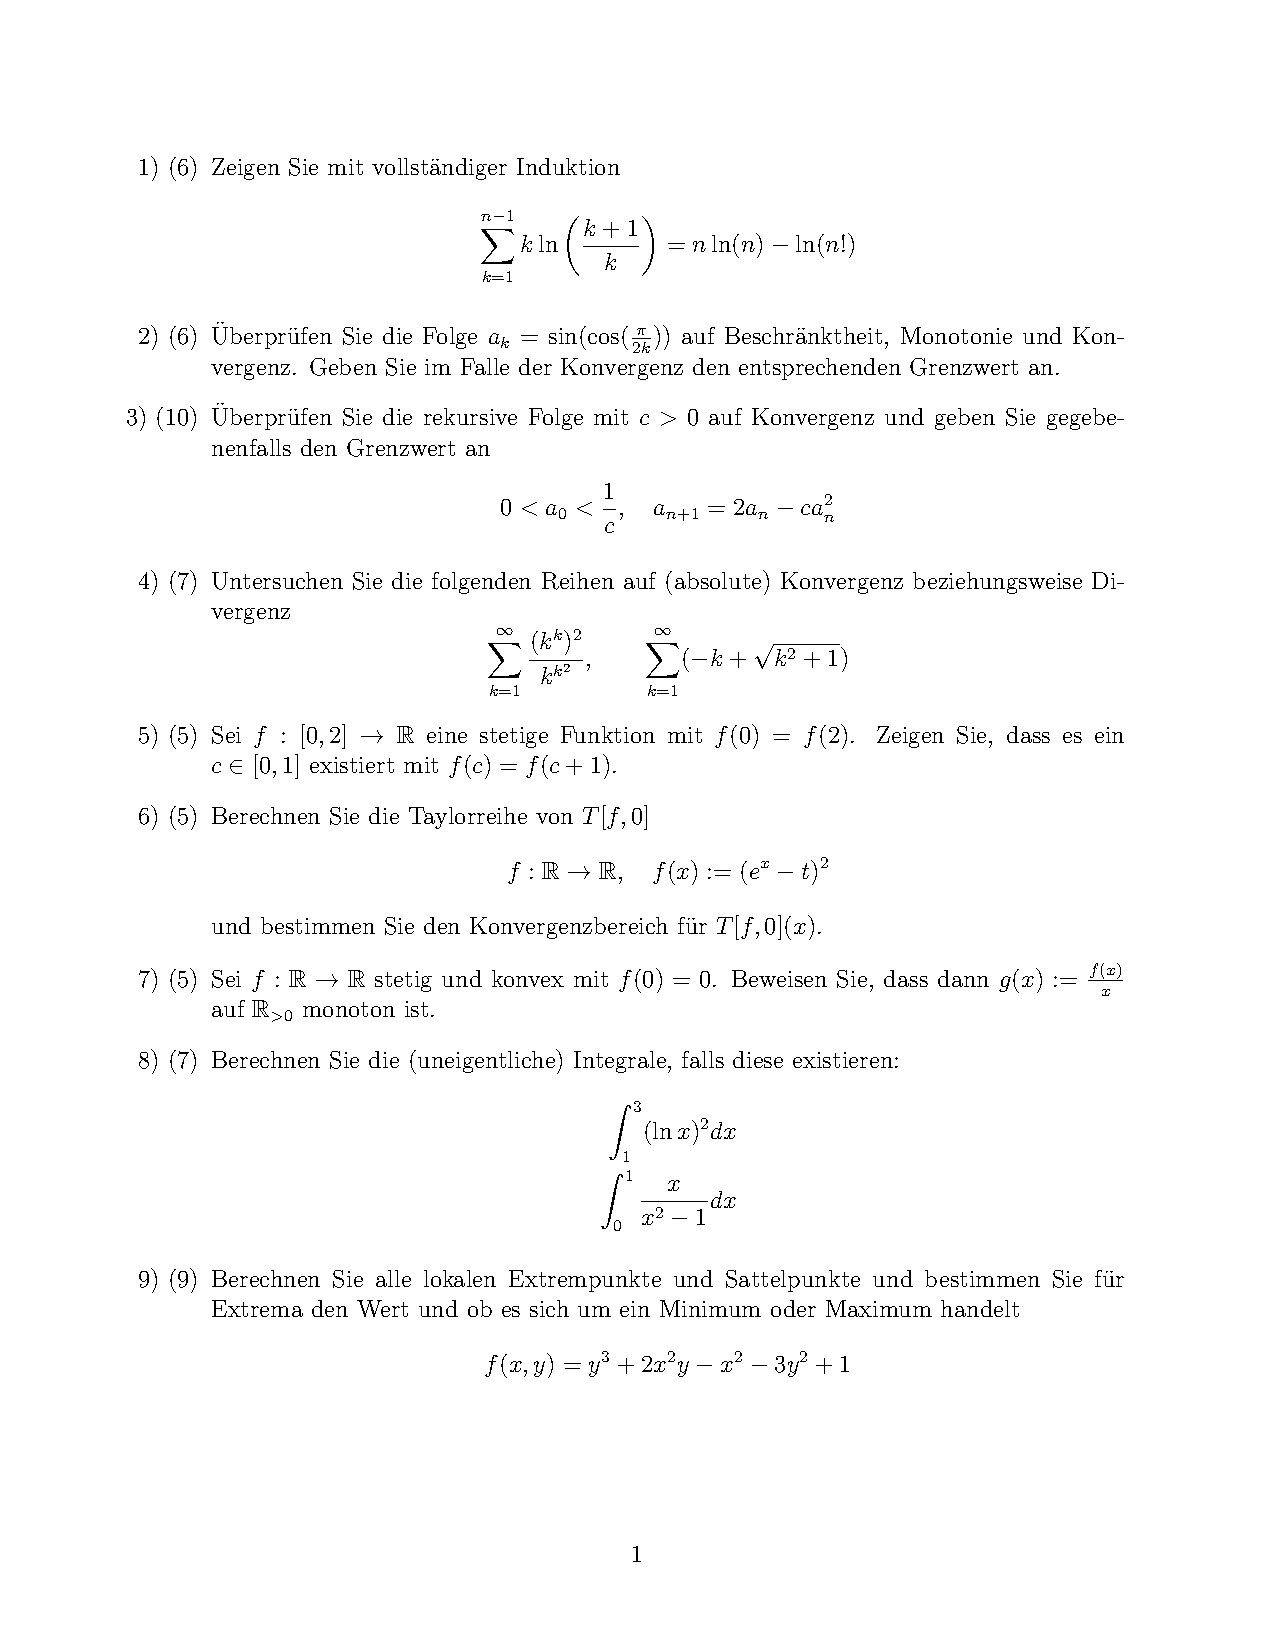
\includegraphics[page=1]{2022.07.05/Probeklausur2.pdf}    

\subsection{Musterlösungsweg Alexander Frank}
\subsubsection{Aufgabe 1}
Induktionsanfang: $(n = 1)$\\
Induktionsvoraussetzung: $\exists n \in \N: A(n)$\\
Induktionsschritt: $(n \rightarrow n+1)$
\begin{align*}
    n\ln(\frac{n+1}{n}) + \sum^{n - 1} ...\\
    \overset{I.V.}{=} n \ln(\frac{n+1}{n}) + n \ln n - \ln (n!)
\end{align*}
Logarithmenregeln
\begin{align*}
    n\cdot \ln(n +1) - \ln(n!)
\end{align*}
+ $0$-Addition
\begin{align*}
    n \cdot \ln(n +1) - \ln (n!) \pm \ln(n+1)
\end{align*}
\subsubsection{Aufgabe 2}
\begin{align*}
    a_k = \sin(\cos(\frac{\pi}{24}))
\end{align*}
\begin{enumerate}[label=\roman*)]
    \item Beschränktheit:$\sin(y_K) \in [-1, 1]$
    \item Monotonie: $z_k = \frac{\pi}{2k} \in [0, \frac{\pi}{2}]$ monoton fallend\\
    $y_k = \cos(z_k)$ monoton steigend\\
    $a_k = \sin(y_k)$ monoton steigend
    \item Konvergenz: Beschränkt + Monoton $\Ra$ Konvergent
    \item Grenzwert: Stetigkeit
    \begin{align*}
        \lim_{n \rightarrow \infty} \sin(\cos(\frac{\pi}{2k})) = \sin(\cos(0)) = \sin(1)
    \end{align*}
\end{enumerate}
\subsubsection{Aufgabe 3}
\begin{enumerate}[label=\roman*)]
    \item Beschränktheit: 
    \begin{align*}
        a_0 \in (0, \frac{1}{c}), a_1 \in (0, \frac{1}{c})
    \end{align*}
    Induktiv zeigen $0 < a_{n} < \frac{1}{c} \forall n \in \N_0$
    \begin{align*}
        0 &< 2a_n - ca_n^2 < \frac{1}{c} &\Leftrightarrow\\
        0 &< \frac{2}{c} a_n - a_n^2 < \frac{1}{c^2} &\Leftrightarrow\\
        0 &< \frac{1}{c^2} - \frac{1}{c^2} + \frac{2}{c}a_n + - a_n ^2 < \frac{1}{c^2} &\Leftrightarrow\\
        0 &< \frac{1}{c^2} - (\frac{1}{c} - a_n)^2 < \frac{1}{c^2}
    \end{align*}
    \item Monotonie: 
    $a_{n+1} \geq a_n \ \forall n \in \N$
    \item Konvergenz: $a = 2a - ca^2$
    \begin{align*}
        a &= 2a - ca^2\\
        ca^2 - a &= 0\\
        ca(a - \frac{1}{c}) &= 0
    \end{align*}
\end{enumerate}
\subsubsection{Aufgabe 4}
a)$\sum_{k=1}^\infty \frac{(k^k)^2}{k^{k^2}}$
\begin{align*}
     \sum_{k=1}^\infty \frac{(k^k)^2}{k^{k^2}} &= \sum_{k=1}^\infty \frac{k^{2k}}{k^{k^2}}
\end{align*}
\begin{align*}
    \lim_{n \rightarrow \infty} \frac{k^2}{k^k} = \frac{1}{k^{k - 2}} \overset{n \rightarrow \infty}{\rightarrow} 0
\end{align*}
b) $\sum_{k=1}^\infty (-k + \sqrt{k^2 + 1})$
\begin{align*}
    \rightarrow \text{3. Binomische Erweiterung} 1- \text{Multiplikation}
\end{align*}
3. Binomische Erweiterung: $\sum (b -  \sqrt{a}) \frac{(b + \sqrt{a})}{b + \sqrt{a}}$
\begin{align*}
    \sum_{k=1}^\infty (-k + \sqrt{k^2 + 1}) &= \sum_{k=1}^\infty \frac{1}{k + \sqrt{k^2 + 1}}
\end{align*}
$\rightarrow $ Minorantenkriterium 
\begin{align*}
    \sum_{k=1}^\infty \frac{1}{k + \sqrt{k^2 + 1}} > \sum_{k=1}^\infty \frac{1}{k + \sqrt{k^2  + k^2}} = \frac{1}{1 + \sqrt{2}} \sum_{k=1}^\infty \frac{1}{k}
\end{align*}
\subsubsection{Aufgabe 5}
Zwischenwertsatz
\begin{align*}
    g(x) := f(x) - f(x + 1)
\end{align*}
$ [0, 1]$ stetig\\
\begin{enumerate}
    \item $f(1) > f(0) $
    \item $f(1) = f(0) $
    \item $f(1) < f(0) $
\end{enumerate}
ZWS $A(x) = B(x) \Rightarrow 0 = A(x) - B(x) $
\subsubsection{Aufgabe 6}
Ableitungen bestimmen\\
$f^{(k)}$ bestimmen: Induktion\\
Tylorreihe bestimmen\\
\begin{align*}
    f(x) = (e^x - t)^2 = e^{2x} - 2te^x +t^2\\
    f'(x) = 2e^{2x} - 2te^x\\
    f''(x) = 2^2 e^{2x} - 2te^x
\end{align*}
\begin{align*}
    \sum_{k = 0}^\infty \frac{f^{(k)}(x_0)}{k!} x^k &= (1 - 2t + t^2) + \sum_{k=1}^\infty ...\\
    &= (1 - 2t + t^2) + \sum_{k = 1}^\infty  \frac{2k - 2t}{k!} x^k
 \end{align*}
\subsubsection{Aufgabe 7}
f stetig, konvex, $f(0) = 0$, $g(x) = \frac{f(x)}{x}$ monoton!\\
\begin{align*}
    f(\lambda x + ( 1 - \lambda) y) \leq \lambda f(x) + (1 - \lambda) f(y)
\end{align*}
$x = 0, y > 0$
\subsubsection{Aufgabe 8}
a)\\
$\rightarrow$ Partielle Integration\\
$\rightarrow$ Stammfunktion $\ln x$\\
b)\\
$\rightarrow$ Substitutionelle Integration
$\rightarrow$ oder kürzen
$\rightarrow$ $1 = \lim_{c \rightarrow 1} c$
\subsubsection{Aufgabe 9}
$f(x, y) = y^3 + 2x^2y + x^2 - 3y^2 + 1$
\begin{enumerate}
    \item Begründe Differenzierbar
    \item Gradient bilden $\Delta f(x, y) = \binom{\delta x f}{\delta y f}$
    \item $\Delta^2 f = Hf = \left(\begin{array}{cc}
        \delta xx &  \delta xy \\
        yx & \delta yy
    \end{array}\right)$
    \item Löse $\delta x f= 0 \land \delta y f = 0$
    (Hier 4 Lösungen)
    \item Punkte in $\sigma^2 f(x_0, y_0)$ $ab - c^2$
\end{enumerate}